\documentclass[letterpaper]{article}
%\usepackage[utf8]{inputenc}
\usepackage[ansinew]{inputenc}
\usepackage[spanish]{babel}
\usepackage{graphicx}

\begin{document}

\title{Anteproyecto1\\ Laboratorio de Microcontroladores}
\author{
 Marco Antonio Montero Chavarr��a Carn�: A94000\\
  \and
  Francisco Molina Carn�: B14194\\  
}
\maketitle

\section{Investigaci�n Previa}
Un sistema de sem�foros inteligente se compone de 2 partes, un sem�foro para el paso de carros que normalmente tiene 3 luces disponibles, rojo para evitar el paso,
amarillo para indicar a los conductores que disminuyan la velocidad ya que el sem�foro est� a punto de cambiar a rojo y verde para indicar paso a los conductores.  Y un segundo sem�foro que esta destinado para los peatones, este posee dos luces, una roja que indica a los peatones que no deben cruzar la calle y el verde que indica que pueden transitar. Cabe destacar que en el caso de los cambios de verde a amarillo  para el sem�foro de autom�viles y el de verde a rojo para el peatonal, se debe poner luz intermitente para avisar que pronto se acabar� el tiempo de paso.\\[0.3 cm]

La idea es disponer de un bot�n de paso en el sem�foro peatonal que al ser presionado, despu�s de un tiempo cambie el estado del sem�foro de autom�viles a un estado de no paso y el sem�foro peatonal a un estado de paso para los peatones. \\[0.3 cm]

Este sistema se utiliza normalmente en la mayor�a de cruces peatonales en el sistema vial. Naturalmente se pretende que si el bot�n de paso no es presionado el sem�foro de autom�viles no cambia de estado ya que ser� innecesario. \\[0.3 cm]

Para este trabajo se tiene un sem�foro de carros un poco m�s simple con solo 2 luces al igual que el peatonal, por lo que es posible recrear la mec�nica de un sem�foro inteligente utilizando las luces disponibles en el microcontrolador stm32f4.


\section{Soluci�n Propuesta}
Utilizando los c�digos de ejemplos del stm32f4 tanto de libopen como de open-coroco, se obtendr�n las herramientas necesarias para el c�digo del sem�foro inteligente. Para ello es de inter�s revisar el manejo de leds, de temporizadores y de operaci�n de botones.

\section{Procedimiento}

Con el esquema de funcionamiento propuesto en la figura \ref{tiempos} y los ejemplos de c�digo se proceder� a elaborar el c�digo paso a paso, atacando el proyecto desde funciones simples hasta lograr el proyecto en su totalidad. 

\begin{figure}[hbtp]
\centering
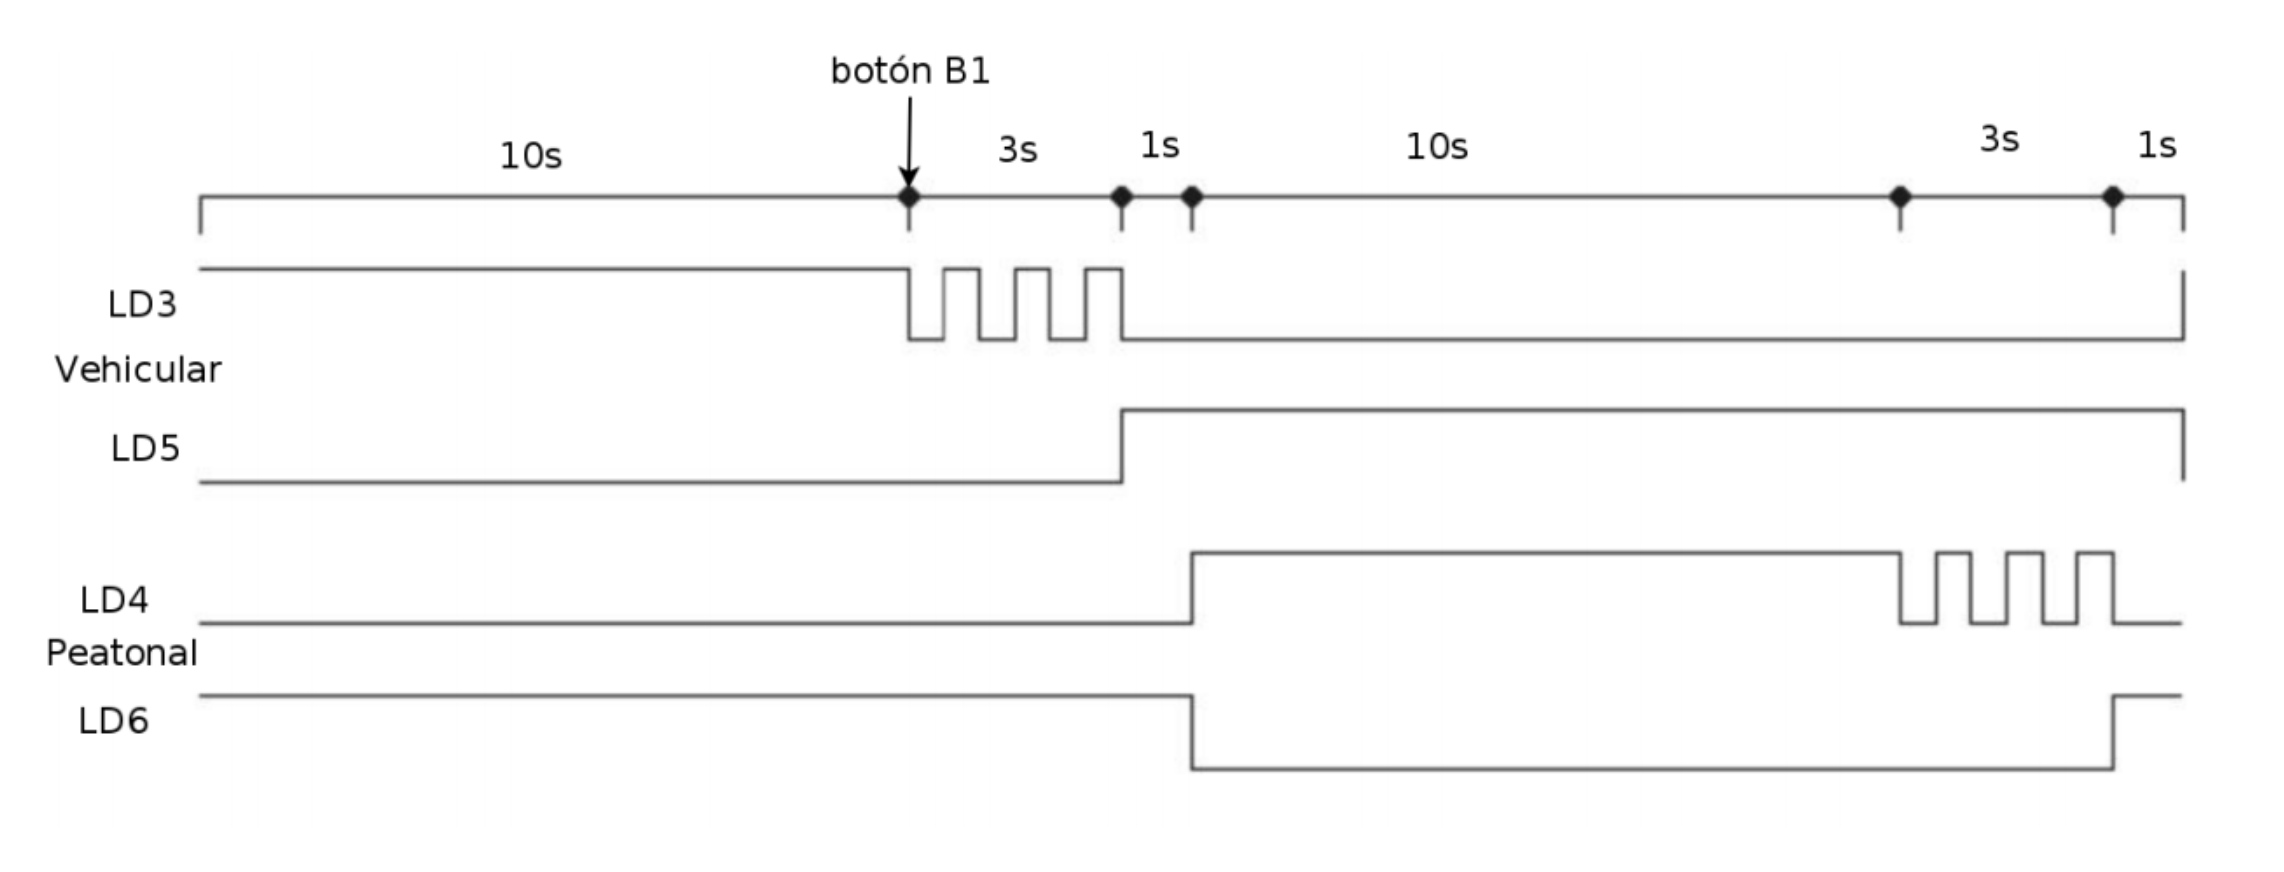
\includegraphics[width=12 cm]{tiempo1.png}
\caption{Diagrama de tiempos}
\label{tiempos}
\end{figure}

Desde esta perspectiva, primero se proceder� a probar el funcionamiento de los LEDs con el programa Miniblink, posteriormente se har� uso de los botones para activar un LED o un programa. Por �ltimo se implementar�n los temporizadores para lograr sincronizar los estados y que todo se ejecute como es debido.

\newpage


\section{Observaciones y recomendaciones}

\begin{itemize}
\item Siempre verificar que la tarjeta responde correctamente con un programa de prueba.
\item Entender el esquema y realizar la m�quina de estados previamente para que se facilite la programaci�n
\end{itemize}



\bibliographystyle{alpha} 
\bibliography{refs}



\end{document}
